\documentclass{phyasgn}
\phyasgn{
  stuname = 姚昊廷,           % 设置学生姓名
  stunum = 22322091,      % 设置学号
  setasgnnum = 3,           % 设置课程次数
  classname = 电磁学,     % 设置课程名称
}

\usepackage{listings}
\usepackage{tikz}
\usepackage{amssymb}
\usepackage{t-angles}
\usepackage{amssymb}
\usepackage{tikz} 
\usetikzlibrary{quotes,angles}
\usetikzlibrary{calc}
\usetikzlibrary{decorations.pathreplacing}
\lstset{numbers=left,basicstyle=\ttfamily,columns=flexible}
\makeatletter
\newcommand{\rmnum}[1]{\romannumeral #1}
\newcommand{\Rmnum}[1]{\expandafter\@slowromancap\romannumeral #1@}
\makeatother


\begin{document}
{\zihao{5}\heiti\color{red} 1-28}
\begin{sol}
设$ne$放在坐标$(0,0,0)$处,$-e$放在坐标$(a,0,0)$处\par
(1)空间中任一点$(x,y,z)$处电势为
$$
\begin{aligned}
    U&=U_1+U_2\\
    &=\frac{e}{4\pi\varepsilon_0}(\frac{n}{\sqrt{x^2+y^2+z^2}}-\frac{1}{\sqrt{(x-a)^2+y^2+z^2}})
\end{aligned}
$$
令$U=0$,则有
$$
\begin{aligned}
    \frac{n}{\sqrt{x^2+y^2+z^2}}-\frac{1}{\sqrt{(x-a)^2+y^2+z^2}}&=0\\
    (x-\frac{n^2a}{n^2-1})^2+y^2+z^2&=(\frac{na}{n^2-1})^2
\end{aligned}
$$\par
(2)该球面球心坐标为$(\frac{n^2a}{n^2-1},0,0)$,符合题意。\par
(3)该球面半径为$\frac{na}{n^2-1}$
\end{sol}\par

{\zihao{5}\heiti\color{red} 1-30}
\begin{sol}
基态氢原子核外电子满足
$$
\frac{e^2}{4\pi\varepsilon_0r^2}=\frac{mv^2}{r}
$$
故动能$E_k=\frac{1}{2}mv^2=\frac{e^2}{8\pi\varepsilon_0r}$,所以氢原子机械能
$W=E_k+E_p=\frac{e^2}{8\pi\varepsilon_0r}+\frac{-e^2}{4\pi\varepsilon_0r}=\frac{-e^2}{8\pi\varepsilon_0r}$
因此电离能
$$
E=-W=2.18\times 10^{-18}J=13.625eV
$$
\end{sol}\par

{\zihao{5}\heiti\color{red} 1-31}
\begin{sol}
(1)$$U=\frac{e}{4\pi\varepsilon_0r}=1.4\times 10^6V$$
$$E_k=e\Delta U=1.4\times 10^6eV$$\par
(2)$$E_k=\frac{3}{2}kT$$
$$T=1.1\times 10^{10}K$$
\end{sol}\par

{\zihao{5}\heiti\color{red} 1-33}
\begin{sol}
(1)
以$O$为势能零点
$$\begin{aligned}
    U_P&=\frac{\eta_e}{2\pi\varepsilon_0}(\ln\frac{a}{\sqrt{(x-a)^2+y^2}}-\ln\frac{a}{\sqrt{(x+a)^2+y^2}})\\
    &=\frac{\eta_e}{4\pi\varepsilon_0}\ln\frac{\sqrt{(x+a)^2+y^2}}{\sqrt{(x-a)^2+y^2}}
\end{aligned}
$$\par
(2)$$
\begin{aligned}
    U&=\frac{\eta_e}{4\pi\varepsilon_0}\ln\frac{\sqrt{(x+a)^2+y^2}}{\sqrt{(x-a)^2+y^2}}\\
    \frac{\sqrt{(x+a)^2+y^2}}{\sqrt{(x-a)^2+y^2}}&=\exp(\frac{4\pi\varepsilon_0U}{\eta_e})=k^2\\
    x^2+2a\frac{k^2+1}{1-k^2}x+a^2+y^2&=0\\
    (x-\frac{k^2+1}{k^2-1}a)^2+y^2&=\frac{4k^2}{(k^2-1)^2}a^2
\end{aligned}
$$
证毕\par
(3)$zOy$平面
\end{sol}\par

{\zihao{5}\heiti\color{red} 1-35}
\begin{sol}
    (1)$$
    \begin{aligned}
        \frac{1}{2}mc^2&=\Delta Ue\\
        U&=\frac{mc^2}{2e}=2.5\times 10^5V
    \end{aligned}
    $$\par
    (2)$$
    \begin{aligned}
        \frac{1}{2}mc^2&=mc^2(\frac{1}{\sqrt{1-\frac{v^2}{c^2}}}-1)\\
        v&=\frac{\sqrt{5}}{3}c=2.2\times 10^8m/s
    \end{aligned}
    $$\par
    (3)$U\to \infty$,不可能
\end{sol}\par

{\zihao{5}\heiti\color{red} 1-39}
\begin{sol}
    (1)取半径为$R$长为$l$的圆柱形高斯面可得
    $$E2\pi Rl=\frac{\int^R_0\frac{\rho_0}{[1+(\frac{r}{a})^2]^2}\mathrm{d}V}{\varepsilon_0}$$
    $$\mathrm{d}V=2\pi rldr$$
    $$E=\frac{\rho_0a^2R}{2\varepsilon_0(a^2+R^2)}$$
    $$E(r)=\frac{\rho_0a^2r}{2\varepsilon_0(a^2+r^2)}$$\par
    (2)$$U(r)=\int_r^0Edr=\frac{\rho_0a^2}{4\varepsilon_0}\ln\frac{a^2}{a^2+r^2}$$
\end{sol}\par


{\zihao{5}\heiti\color{red} 1-41}
\begin{sol}
    由场强叠加原理知
    $$E=\left\{\begin{matrix}
        0&(x<-\frac{d}{2}) \\
        \frac{\sigma_e}{\varepsilon_0} &(-\frac{d}{2}<x<\frac{d}{2}  ) \\
        0&(x>\frac{d}{2} )
      \end{matrix}\right.$$
      又因为$O$处电势为0
      $$U(x)=\int_x^0-E\mathrm{d}x=\frac{\sigma_e}{\varepsilon_0}x$$
      其$E-x$与$U-x$图为
      \begin{figure}[htbp]
        \begin{tikzpicture}
            \draw[->] (-5,0) --(5,0) node[right]{$x$};
            \draw[->] (0,-5) --(0,5) node[right]{$E$};
            \draw[loosely dashed] (-1,5) --(-1,0)node[below]{$-\frac{d}{2}$};
            \draw[loosely dashed] (1,5) --(1,0)node[below]{$\frac{d}{2}$};
            \draw (-1,3) --(1,3);
            \node at(0.3,3) {$\frac{\sigma_e}{\varepsilon_0}$};
        \end{tikzpicture}
    \end{figure}
    \begin{figure}[!h]
        \begin{tikzpicture}
            \draw[->] (-5,0) --(5,0) node[right]{$x$};
            \draw[->] (0,-5) --(0,5) node[right]{$U$};
            \draw[loosely dashed] (-1,5) --(-1,0)node[below]{$-\frac{d}{2}$};
            \draw[loosely dashed] (1,5) --(1,0)node[below]{$\frac{d}{2}$};
            \draw[loosely dashed] (-1,0) --(-1,-5);
            \draw[loosely dashed] (1,0) --(1,-5);
            \draw (-1,-3) --(1,3);
            \draw[loosely dashed] (1,3) --(0,3)node[left]{$\frac{\sigma_e d}{2\varepsilon_0}$};
            \draw (-1,-3) --(-5,-3);
            \draw (1,3) --(5,3);
        \end{tikzpicture}
      \end{figure}
\end{sol}\newpage

{\zihao{5}\heiti\color{red} 1-43 }
\begin{sol}
    (1)由高斯定理
    $$
    \begin{aligned}
        E\cdot S&=\frac{S}{\varepsilon_0}\int_{-x_N}^{X}\rho\mathrm{d}x\\
        E&=\frac{ea}{8\varepsilon_0}(x_m^2-4x^2)
    \end{aligned}
    $$
    \begin{figure}[!h]
        \begin{tikzpicture}
            \draw[->] (-5,0) --(5,0) node[right]{$x$};
            \draw[->] (0,-5) --(0,5) node[right]{$\rho$};
            \draw[loosely dashed] (-1,5) --(-1,0)node[below]{$-\frac{x_m}{2}$};
            \draw[loosely dashed] (1,5) --(1,0)node[below]{$\frac{x_m}{2}$};
            \draw[loosely dashed] (-1,0) --(-1,-5);
            \draw[loosely dashed] (1,0) --(1,-5);
            \draw (-1,3) --(1,-3);
            
        \end{tikzpicture}
      \end{figure}
      \begin{figure}[!h]
        \begin{tikzpicture}
            \draw[->] (-5,0) --(5,0) node[right]{$x$};
            \draw[->] (0,-5) --(0,5) node[right]{$E$};
            \draw[loosely dashed] (-1,5) --(-1,0)node[below]{$-\frac{x_m}{2}$};
            \draw[loosely dashed] (1,5) --(1,0)node[below]{$\frac{x_m}{2}$};
            \draw[loosely dashed] (-1,0) --(-1,-5);
            \draw[loosely dashed] (1,0) --(1,-5);
            \draw[domain =-1:1] plot (\x ,{1-\x*\x}) ;
            
        \end{tikzpicture}\par
        (2)令$U=0$,则$x=0$,该电势以原点为零点,$\Delta U=U(\frac{x_m}{2})-U(-\frac{x_m}{2})=-\frac{eax_m^2}{12\varepsilon_0}$

      \end{figure}
\end{sol}\newpage

{\zihao{5}\heiti\color{red} 1-44 }
\begin{sol}
  同一电场线上任取AB两点,过AB两点作底面积无限小的柱形高斯面,因为该面中无电荷
  $E_AS=E_BS$故$E_A=E_B$,在不同电场线任取AC作闭合矩形回路,因为场强环路积分为0,故
  $E_Al=E_Cl$,故$E_A=E_C$,又因为ABC均是任取的,故处处场强相等。
\end{sol}\par

{\zihao{5}\heiti\color{red} 附加题1}
\begin{sol}
    \begin{figure}[!h]
        \begin{tikzpicture}
            \coordinate (p) at (3,4);
            \coordinate (o) at (0,0);
            \coordinate (a) at (1,0);
            \coordinate (b) at (-1,0);
            \draw[->] (-5,0) --(5,0) node[right]{$x$};
            \draw[->] (0,-5) --(0,5) node[right]{$y$};
            \draw[->] (1,0) --(1,-1) node[below]{$\vec{p}_1$};
            \draw[->] (-1,0) --(-1,1) node[above]{$\vec{p}_2$};
            \draw[->] (o) --(p) node[right]{$P(r,\theta)$};
            \draw[->] (a) --(p) ;
            \draw[->] (b) --(p) ;
            \node at(2,1) {$\vec{r}_1$};
            \node at(1,2.5) {$\vec{r}_2$};
            \pic["$\theta$", draw=red!40, <->, angle eccentricity=0.6, angle radius=0.7cm]
            {angle=a--o--p};
        \end{tikzpicture}
    \end{figure}
    该电四极子可视为两个电偶极子叠加,其电偶极距分别为$\vec{p}_1$,$\vec{p}_2$
    $$
    \begin{aligned}
        U_1&=\frac{\vec{p}_1\cdot \vec{r}_1}{4\pi\varepsilon_0 r_1^3}\\
        &=\frac{-rql\sin\theta}{4\pi\varepsilon_0}\frac{1}{(r^2+\frac{l^2}{4}-rl\cos\theta)^\frac{3}{2}}
    \end{aligned}
    $$

    $$
    \begin{aligned}
        U_2&=\frac{\vec{p}_2\cdot \vec{r}_2}{4\pi\varepsilon_0 r_2^3}\\
        &=\frac{rql\sin\theta}{4\pi\varepsilon_0}\frac{1}{(r^2+\frac{l^2}{4}+rl\cos\theta)^\frac{3}{2}}
    \end{aligned}
    $$

    $$
    \begin{aligned}
        U_P&=U_1+U_2\\
        &=\frac{-rql\sin\theta}{4\pi\varepsilon_0}[\frac{1}{(r^2+\frac{l^2}{4}-rl\cos\theta)^\frac{3}{2}}-\frac{1}{(r^2+\frac{l^2}{4}+rl\cos\theta)^\frac{3}{2}}]
    \end{aligned}
    $$
    因为$l \ll r$,故略去二阶小量$\frac{l^2}{4}$,且运用近似$(1+x)^k= 1+kx(x\ll 1)$可得
    $$
    U_P=\frac{-rql\sin\theta}{4\pi\varepsilon_0}(\frac{1+\frac{3}{2}\frac{l\cos\theta}{r}-1+\frac{3}{2}\frac{l\cos\theta}{r}}{r^3})=\frac{-3ql\sin\theta\cos\theta}{4\pi\varepsilon_0r^3}
    $$
\end{sol}\par

{\zihao{5}\heiti\color{red} 附加题2}
\begin{sol}
    \begin{figure}[!h]
        \begin{tikzpicture}
            \coordinate (p) at (3,4);
            \coordinate (o) at (0,0);
            \coordinate (a) at (1,0);
            \coordinate (b) at (-1,0);
            \draw[->] (-5,0) --(5,0) node[right]{$x$};
            \draw[->] (0,-5) --(0,5) node[right]{$y$};
            \draw[->] (1,0) --(2,0) node[right]{$\vec{p}_1$};
            \draw[->] (-1,0) --(-2,0) node[left]{$\vec{p}_2$};
            \draw[->] (o) --(p) node[right]{$P(r,\theta)$};
            \draw[->] (a) --(p) ;
            \draw[->] (b) --(p) ;
            \node at(2,1) {$\vec{r}_1$};
            \node at(1,2.5) {$\vec{r}_2$};
            \pic["$\theta$", draw=red!40, <->, angle eccentricity=0.6, angle radius=0.7cm]
            {angle=a--o--p};
        \end{tikzpicture}
    \end{figure}
    该电四极子可视为两个电偶极子叠加,其电偶极距分别为$\vec{p}_1$,$\vec{p}_2$
    $$
    \begin{aligned}
        U_1&=\frac{\vec{p}_1\cdot \vec{r}_1}{4\pi\varepsilon_0 r_1^3}\\
        &=\frac{1}{4\pi\varepsilon_0}\frac{r\cos\theta ql-\frac{ql^2}{2}}{(r^2+rl\cos\theta+\frac{l^2}{4})^{\frac{3}{2}}}
    \end{aligned}
    $$

    $$
    \begin{aligned}
        U_2&=\frac{\vec{p}_2\cdot \vec{r}_2}{4\pi\varepsilon_0 r_2^3}\\
        &=\frac{1}{4\pi\varepsilon_0}\frac{r\cos\theta ql+\frac{ql^2}{2}}{(r^2+rl\cos\theta-\frac{l^2}{4})^{\frac{3}{2}}}
    \end{aligned}
    $$

    $$
    \begin{aligned}
        U_P&=U_1+U_2\\
        &=\frac{r\cos\theta ql}{4\pi\varepsilon_0r^3}[(r\cos\theta ql-\frac{ql^2}{2})(1+\frac{3l\cos\theta}{2r})-(r\cos\theta ql+\frac{ql^2}{2})(1-\frac{3l\cos\theta}{2r})]\\
        &=\frac{ql^2(3\cos^2\theta-1)}{4\pi\varepsilon_0r^3}=\frac{D(3\cos^2\theta-1)}{8\pi\varepsilon_0r^3}
    \end{aligned}
    $$
    $$
    \begin{aligned}
        \vec{E}&=-\nabla U\\
        &=-\frac{\partial U}{\partial r}\hat{e}_r-\frac{\partial U}{r\partial \theta}\hat{e}_\theta\\
        &=\frac{3ql^2}{4\pi\varepsilon_0r^4}[(3\cos^2\theta-1)\hat{e}_r+2\sin\theta\cos\theta\hat{e}_\theta]
    \end{aligned}
    $$
    电场线如图
    \begin{figure}[!h]
        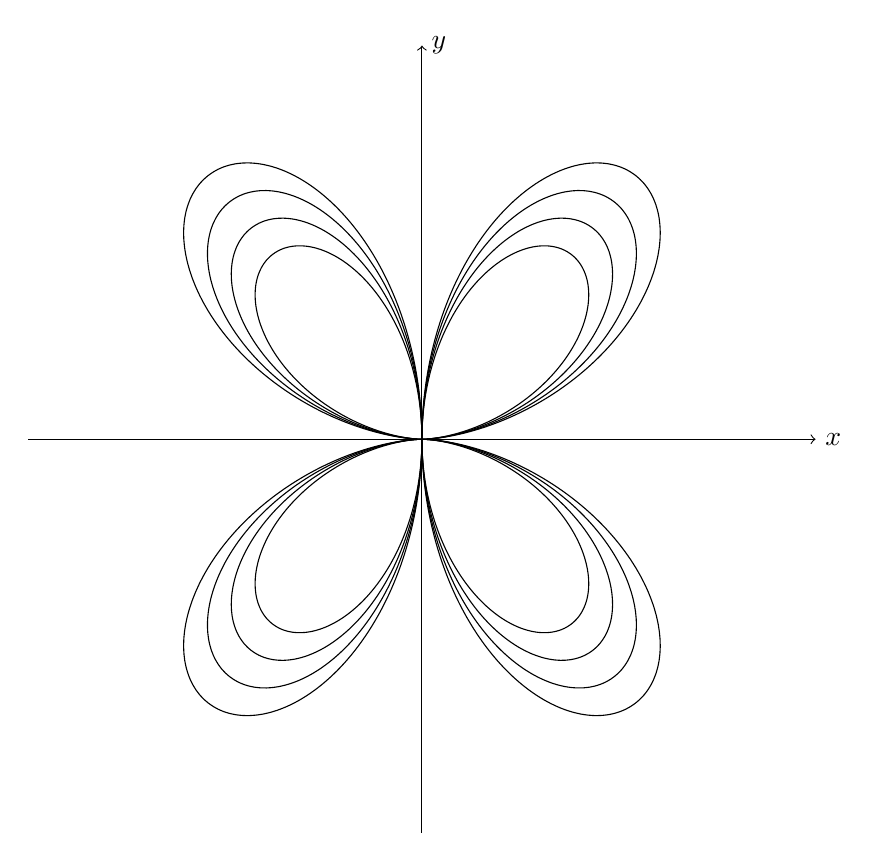
\begin{tikzpicture}
            \draw[->] (-5,0) --(5,0) node[right]{$x$};
            \draw[->] (0,-5) --(0,5) node[right]{$y$};
            \draw[domain=0:180,samples=1000] plot (\x:{10*sqrt{sin(\x)*sin(\x)*cos(\x)}});
            \draw[domain=0:180,samples=1000] plot (\x:{-10*sqrt{sin(\x)*sin(\x)*cos(\x)}});
            \draw[domain=0:180,samples=1000] plot (\x:{9*sqrt{sin(\x)*sin(\x)*cos(\x)}});
            \draw[domain=0:180,samples=1000] plot (\x:{-9*sqrt{sin(\x)*sin(\x)*cos(\x)}});
            \draw[domain=0:180,samples=1000] plot (\x:{8*sqrt{sin(\x)*sin(\x)*cos(\x)}});
            \draw[domain=0:180,samples=1000] plot (\x:{-8*sqrt{sin(\x)*sin(\x)*cos(\x)}});
            \draw[domain=0:180,samples=1000] plot (\x:{7*sqrt{sin(\x)*sin(\x)*cos(\x)}});
            \draw[domain=0:180,samples=1000] plot (\x:{-7*sqrt{sin(\x)*sin(\x)*cos(\x)}});
            \end{tikzpicture}
        
        
    \end{figure}
\end{sol}\par
\end{document}